\section{Definition}
\label{sec:definition}
\noindent\textbf{World.}
We define the \emph{world} as the set of task-relevant entities under consideration. Its scope is not fixed, but depends on the task or modeling objective. For example, in an inverted-pendulum control problem, the world may consist only of the pendulum system. In robotic manipulation, the world typically includes the robot itself, the objects it needs to interact with, and the surrounding environment that may affect task execution. For a model that aims to capture broad physical regularities across objects, scenes, and interactions, the world may further extend to the physical environment at large. In this sense, the world is a task-dependent abstraction that specifies what entities are considered relevant.


\noindent\textbf{World Model.}
Given a \emph{world}, we define a \emph{world model} as a model that captures how task-relevant aspects of the world evolve under actions. Since the true state of the world is often not directly or fully observable, this evolution is typically modeled from observations. Let $o_t$ denote an observation of the world at time $t$, such as an RGB or RGB-D image, a point cloud, or a robot proprioceptive state, and let $a_t$ denote the action applied at that time, which may range from a concrete agent action to an abstract language-level action or a camera pose for observing the environment.

Depending on the prediction target, world models can be formulated either in observation space or in state space, as illustrated in Fig.~\ref{fig:overview}. For clarity, we first present the one-step formulation, while the same formulation naturally extends to multi-step prediction. An observation-space world model predicts the next observation,
\[
o_{t+1} \sim p(\cdot \mid o_{0:t}, a_t),
\]
where the target is a future observation. In contrast, a state-space world model predicts a future state or representation of interest,
\[
x_{t+1} \sim p(\cdot \mid o_{0:t}, a_t),
\]
where $x_{t+1}$ may correspond to object poses, keypoints, latent states, or other task-relevant quantities. More generally, the target can be a future trajectory, such as $o_{t+1:t+H}$ or $x_{t+1:t+H}$. These formulations also cover common special cases: in Markovian settings, the observation history $o_{0:t}$ can be summarized by the current observation $o_t$; in deterministic settings, the predictive distribution reduces to a deterministic transition.


\begin{figure}[t]
    \centering
    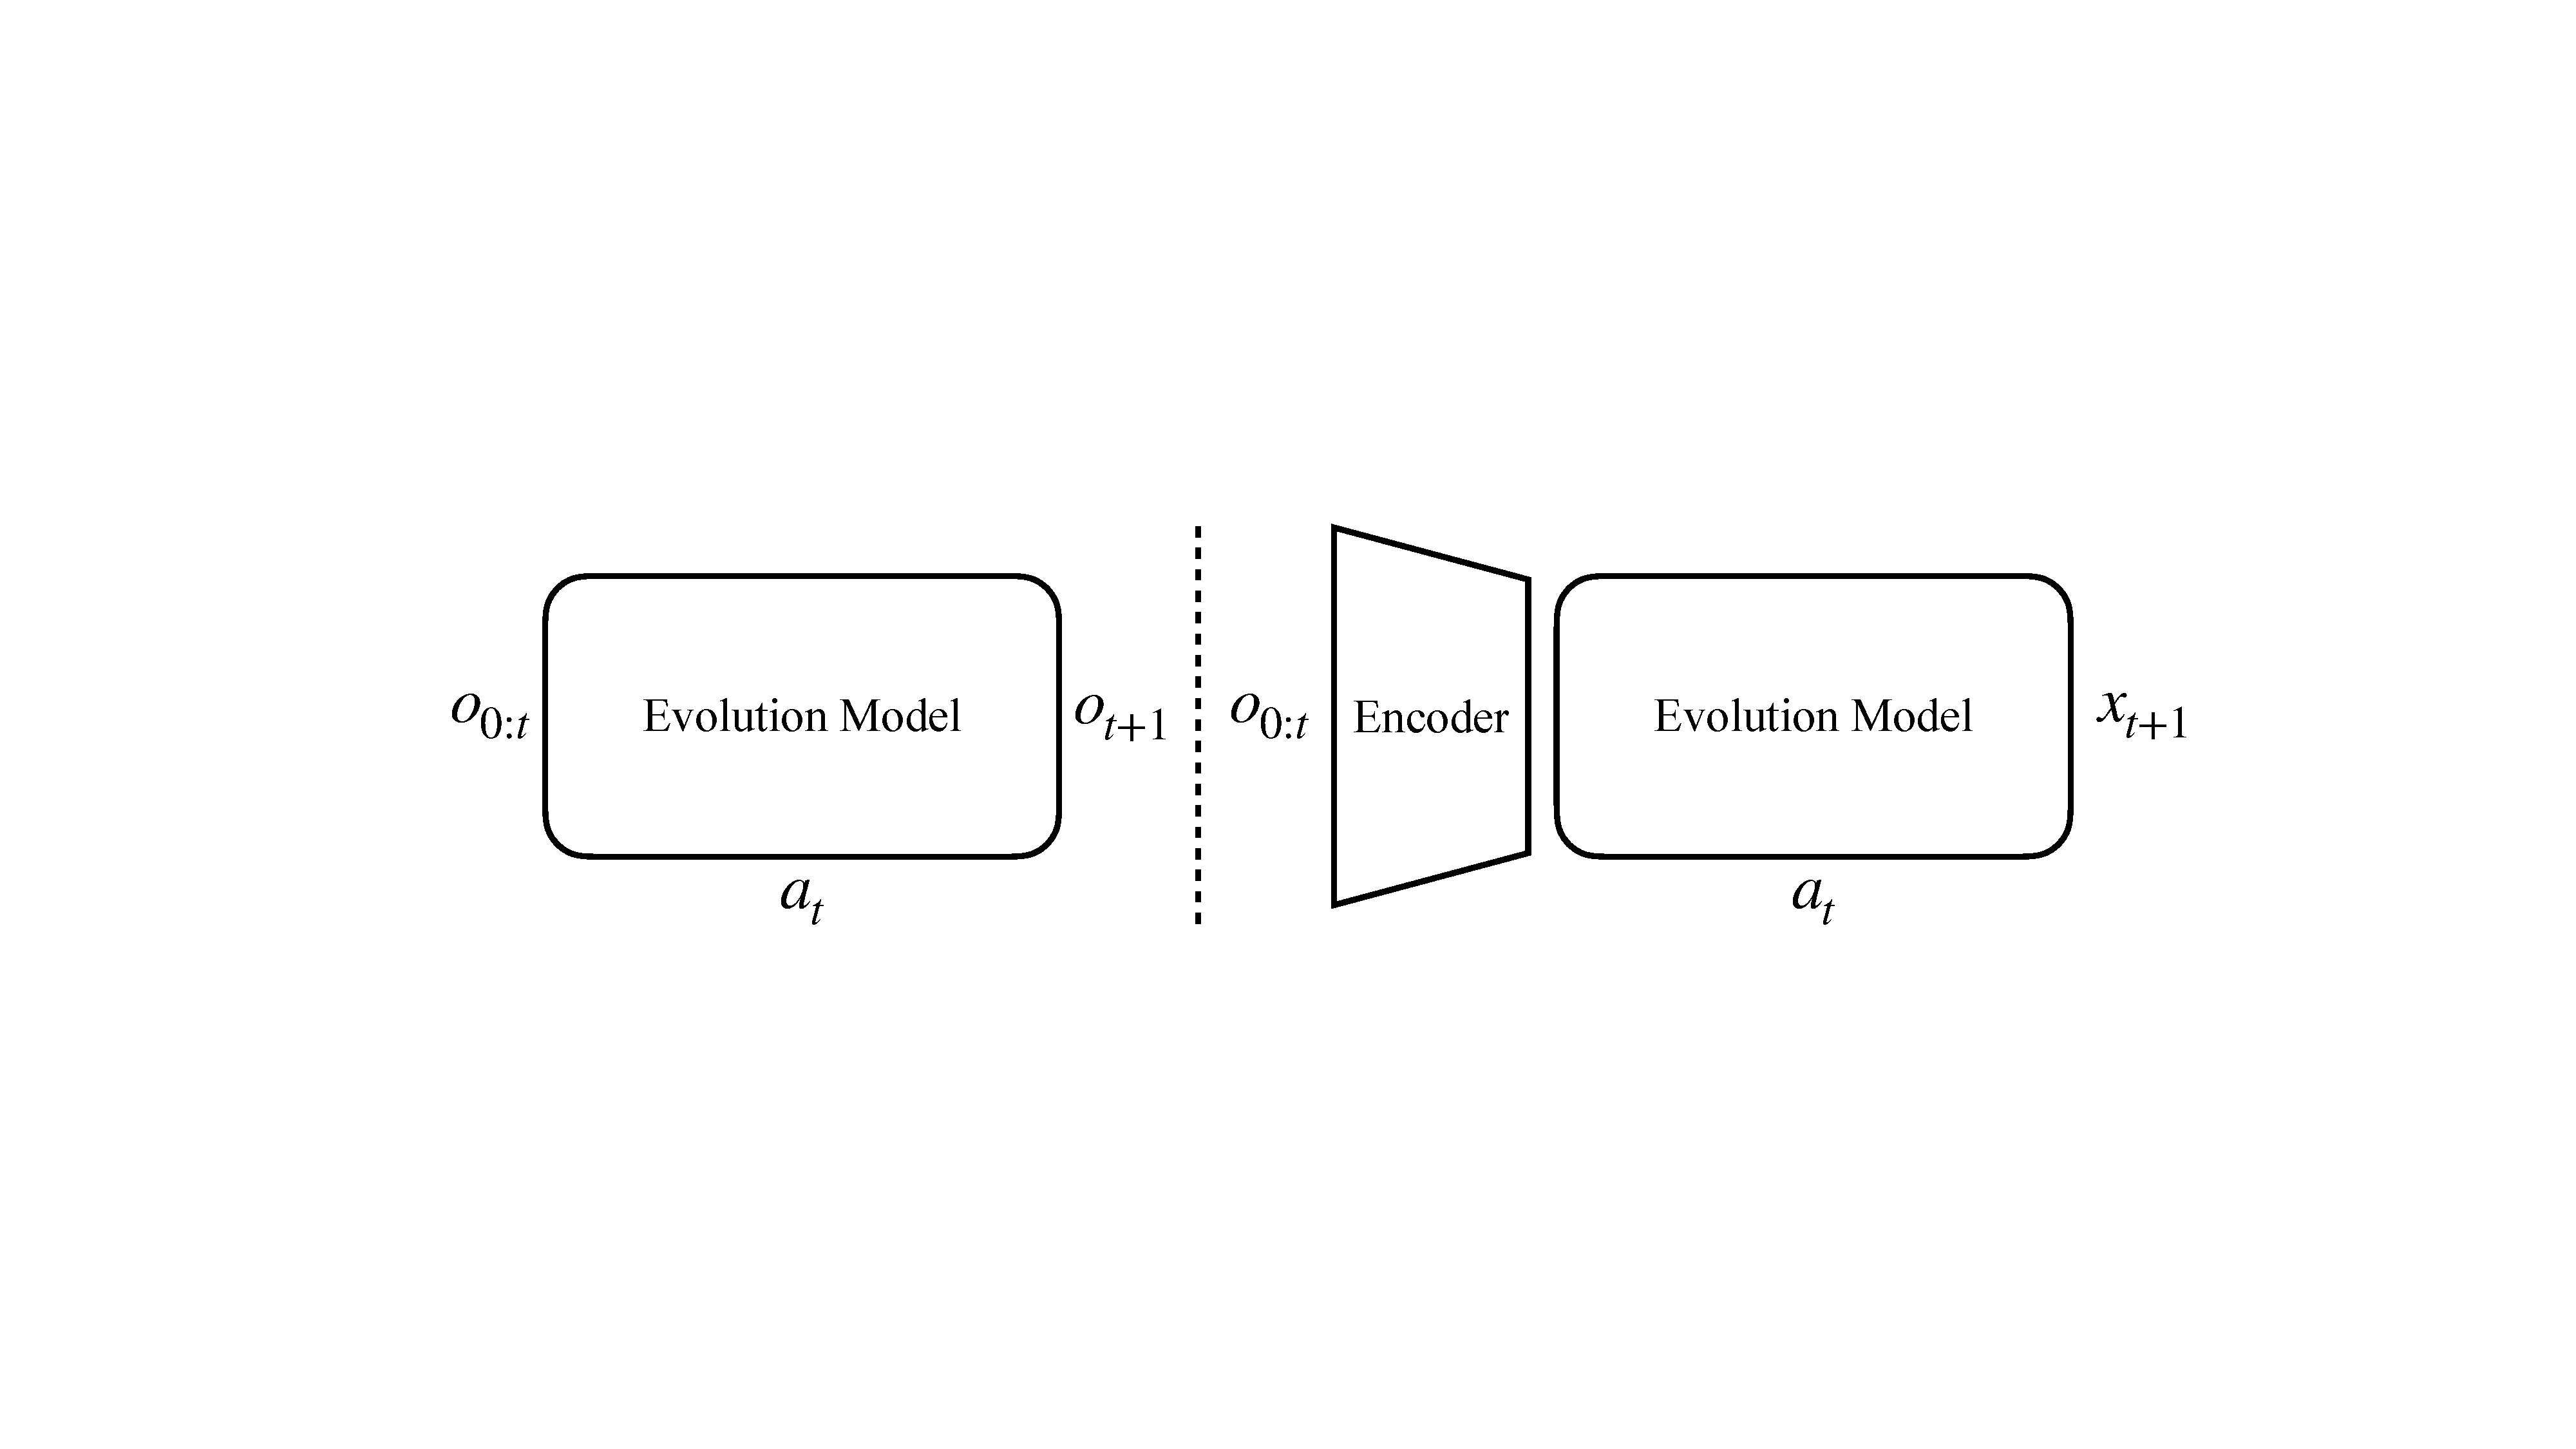
\includegraphics[width=0.98\linewidth]{figs/overview.pdf}
    \caption{Two formulations of world models. \textbf{Left:} an observation-space world model directly predicts the future observation $o_{t+1}$ from the observation history $o_{0:t}$ and action $a_t$. \textbf{Right:} a state-space world model first encodes $o_{0:t}$ into an internal representation, and then uses an evolution model conditioned on $a_t$ to predict the future quantity of interest $x_{t+1}$.}

    \label{fig:overview}
\end{figure}
